\documentclass[10pt,a4paper]{article}
\usepackage[utf8]{inputenc}
\usepackage[german]{babel}
\usepackage[T1]{fontenc}
\usepackage{amsmath}
\usepackage{amsfonts}
\usepackage{amssymb}
\usepackage[official]{eurosym}

\usepackage{wrapfig}

\usepackage{graphicx}
\graphicspath{ {./} }


\begin{document}

\begin{center}


\includegraphics[scale=.75]{logo.jpg}
\end{center}

\begin{flushright}
runIT business GmbH \\
Römerstraße 7\\
54295 Trier\\
Tel.: 0651 / 99 55 60\\
Fax: 0651 / 99 55 61\\
Mail: info@runit.de\\
www.runit.de\\
\end{flushright}

\begin{flushleft}
Universität Trier\\
z.Hd.: Dr. habil. Axel Kalenborn \& M. Sc. Colja Becker\\
Campus II, Raum H 309\\
Behringstraße 21\\
54296 Trier\\
\end{flushleft}

\begin{flushright}
Trier, den 20.01.2016
\end{flushright}

\tableofcontents

\section{Unternehmensdarstellung}
Die runIT business GmbH ist ein im Jahr 2012 gegründetes Unternehmen. Wir haben es uns seitdem als IT-Dienstleister zur Aufgabe gemacht, für unsere Kunden qualitativ hochwertige und individuelle Softwarelösungen zu entwickeln. Von der Softwareentwicklung bis hin zur Softwareeinführung bieten wir Ihnen das komplette Leistungsspektrum eines IT-Dienstleisters und berücksichtigen branchenspezifische sowie individuelle Anforderungen und Wünsche unserer Kunden. 

Seit der Unternehmensgründung im Jahr 2012 beschäftigt die runIT business GmbH heute 14 erfahrene IT-Experten der verschiedensten Technologien. Durch die Erfahrung und Leidenschaft unserer Mitarbeiter ist es uns möglich Ihnen innovative Softwarelösungen für komplexe Prozesse sowie effizientere Abläufe Ihres Business zu liefern. 

\section{Projektteam}
Zur Konzeption und Entwicklung des LMS-Systems planen wir folgende Zusammensetzung unseres Projektteams:

\begin{center}
	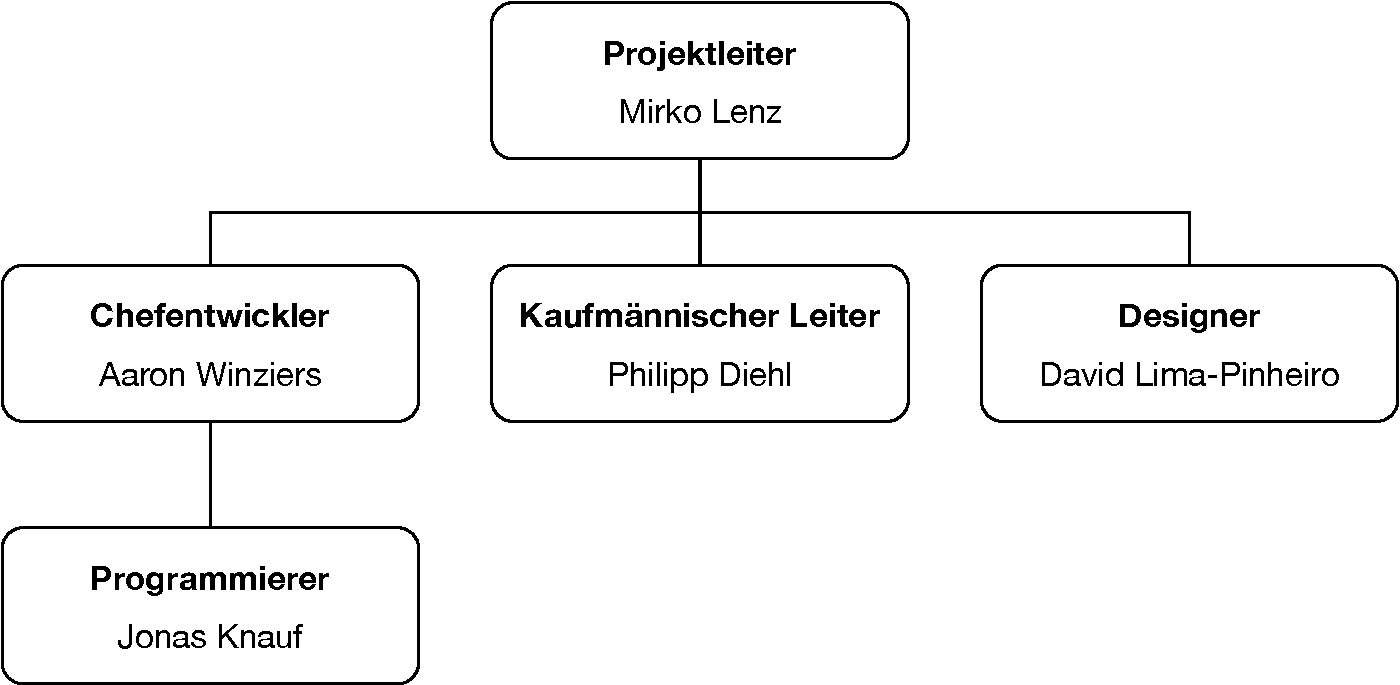
\includegraphics[scale=.4]{Gruppeneinteilung.pdf}
\end{center}

Der Projektleiter Herr Mirko Lenz ist als ehemalige wissenschaftliche Hilfskraft des RWP-Lehrstuhl der Universität Trier mit den Systemen der Universität Trier vertraut. Des Weiteren greift er auf die Erfahrung verschiedener Prijekte mit der Unternehmensberatung KPMG auf. Auch als Head of Sales bei Contact \& Cooperation sammelte er Erfahrung in der Projektleitung.

Herr Aaron Winziers wird als Chefentwickler zusammen mit unserem Programmierer, Herr Jonas Knauf, für die Entwicklung und Implementierung des LMS-Systems zuständig sein. Unser erfahrener Chefentwickler arbeitete im Rahmen eines Studienprojekts mit dem IPv6 Netzwerkprotokoll und bringt Erfahrungen aus der Teilnahme bei der Umsetzung eines elektronischen Akten-Systems bei der Carl Zeiss AG mit. Herr Knauf kann eine umfangreiche Erfahrung aus verschiedenen Programmierprojekten sowie einem Praktikum bei der Arla Foods Deutschland GmbH aufweisen. Zudem betreibt er einen Web-Server.

Unsere kaufmännische Leitung Herr Philipp Diehl ist für das Controlling sowie die Kundenbetreuung verantwortlich. Auch er bringt zahlreiche Erfahrungen in der Angebotserstellung eines Maschinenbau-Unternehmens mit sowie der Entwicklung und Ausarbeitung eines Marketingkonzepts mit Servicepaketen. Zudem war er im Rahmen eines Forschungsprojekts an der Erstellung eines Business Plans für die Ausgliederung einer CRM-Software für die Cursor Software AG beteiligt.

\section{Referenzprojekte}
Mit der runIT business GmbH haben Sie einen erfahrenen IT-Partner an Ihrer Seite. Im Folgenden möchten wir Ihnen kurz einige ausgewählte Projekte vorstellen, die die runIT business GmbH zur Zufriedenheit Ihrer Kunden konzipierte und erfolgreich realisieren konnte.

 
Für die Insearch Group konzipierte und entwickelte die runIT business GmbH ein individuelles Datenbankmanagementsystem zur Optimierung von Recruiting- und Bewerbungsprozessen. Das auf die Wünsche der Insearch Group angepasste Datenbankmanagementsystem ermöglicht die Verwaltung komplexer Bewerber- und Kundendaten und stellt den Mittelpunkt der Tätigkeiten der Insearch Group dar. Durch die nutzerfreundliche Übertragung der Bewerberdaten wird der Arbeitsalltag der Mitarbeiter der Personalberatung erleichtert und die Prozesse im Unternehmen optimiert.

Volksfreund-Druckerei Nikolaus Koch GmbH
Gemeinsam mit der Volksfreund-Druckerei Nikolaus Koch GmbH konzipierte ein Projektteam der runIT business GmbH ein neues Customer-Relationship-Management System. Dieses CRM-System ermöglicht sowohl eine zentrale Verwaltung der Kundendaten der Abonnements als auch die Verwaltung der Online-Kunden. Neue Kundendaten können somit von den Mitarbeitern der unterschiedlichen Abteilungen der Volksfreund-Druckerei Nikolaus Koch GmbH auf nutzerfreundlicher Weise integriert und aufbereitet werden.

\section{Funtionale Realisierung des Projekts}
\subsection{Studierende/Partner mit Kontakthistorie}
Auf der Seite "Studierende" findet sich eine Liste mit allen Studierenden. Laut Lastenheft sollte eine solche Liste zwar auf der Startseite zu finden sein, wir haben uns jedoch aus Komfortgründen für eine andere Variante entschieden. Oft verwaltet ein Mitarbeiter seine bisherigen Kontakt oder möchte einen neuen Kontakt mit einem ihm bisher unbekannten Studierenden anlegen. Auf der Startseite findet er so eine schnelle Möglichkeit, seine derzeitigen Kontakte zu verwalten. Eine vollständige Liste müsste in mehreren Schritten gefiltert und sortiert werden, um zum gewünschten Ergebnis zu gelangen. Hier sieht er auf einen Blick relevante Kontakte und kann mit nur einem Klick zu einer Suchleiste und einem allgemeinen Verzeichnis gelangen. Eine solche Lösung erlaubt es darüber hinaus, die Startseite im Laufe der Zeit flexibel mit neuen Sichten auszustatten.


\subsection{Funktionale Anforderungen}
\subsubsection{Sichten}
\begin{itemize}
	\item Login
	\item Startseite
	\begin{itemize}
		\item letzte eigene Kontakte mit Studierenden
		\item Heutige Termine
	\end{itemize}
	\item Studierende \& Partner
	\begin{itemize}
		\item Liste alle Studierenden
		\item Freitextsuche
		\item Erweiterte Suche
		\item Kontakthistorie
		\item Nachricht senden
		\item Stammdaten
		\item Neuer Termin
		\item Drucken
		\item Zukünftige Termine exportieren
		\item nur für Partner: Neu anlegen
	\end{itemize}
	\item Arbeiten
	\begin{itemize}
		\item Neue Arbeit anlegen
		\item Freitextsuche
		\item Erweiterte Suche
		\item Liste aller Arbeiten
	\end{itemize}
\end{itemize}

\subsubsection{Funktionen}
\begin{itemize}
	\item Login über Mitarbeitertabelle
	\item Sortierung und Filterung aller Listen
	\item Suche in Datenbank
	\item Nachricht senden
	\item Stammdaten anzeigen
	\item Neuen Termin anlegen
	\item Historie drucken
	\item Export der Termine
	\item neue Partner/Arbeiten anlegen
\end{itemize}


\subsubsection{Struktur der Datenbank}
\hspace{-60pt}
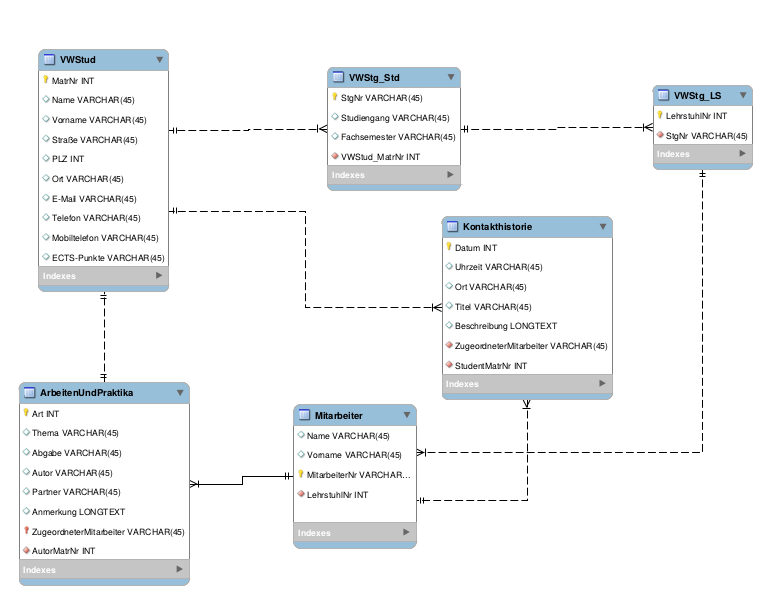
\includegraphics[scale=.75]{Datenbank.png}

\section{Qualitätsanforderungen}
Ihre Zufriedenheit ist für uns ein großes Anliegen. Daher haben wir strenge Qualitätsanforderungen an die Software, bevor diese unser Haus verlässt.

Die Performanz des LMS muss zu jeder Zeit gewährleistet sein. So dürfen zwischen dem Aufruf des Benutzers, der Anfrage an die Datenbank und dem anschließenden Download des Quellcodes maximal 500 Millisekunden vergehen. Dies stellen wir durch effiziente Algorithmen und Ping-Tests an Webseite und Datenbank sicher.

Die Zuverlässigkeit garantieren wir durch den Einsatz bewährter und qualifizierter Komponenten. Wir führen Stresstests durch, um das System umfassend zu überprüfen. Selbst für den unwahrscheinlichen Fall, dass alle etwa 1000 Vollzeitbeschäftigte der Universität Trier gleichzeitig online sind, hat unser System noch Reserven.

Sicherheit spielt in unserem Umfeld ebenfalls eine sehr große Rolle. Wir verwenden moderne Kompatibilität mittels TLS als Verschlüsselungsprotokoll und speichern die Passwörter auf Ihren Wunsch über das SHA-1 Hash-Verfahren. Zusätzlich führen wir einen Penetrationstest durch, um mögliche Schwachstellen frühzeitig zu erkennen und beseitigen.

\section{Zeit und Ressourcenplanung}
Aufbauend auf die Anforderungen im Lastenheft der Ausschreibung haben wir folgende Zeitplanung für das Projekt der Entwicklung eines LMS-Systems für die Universität Trier erstellt.

Grafik der Zeitplanung so in etwa wie in der Excel-Datei.

Laut Lastenheft erfolgt die Vergabe des Projekts am 6. Februar 2017. Darauf folgend sieht die Zeitplanung der runIT business GmbH für das Projekt eine Fertigstellung der Konzeption und Entwicklung der Datenstruktur bis zum 15. Februar vor. Aufbauend auf der Konzeption und Entwicklung der Datenstruktur planen wir mit der Umsetzung des Java-Frameworks für die Sichten der Kontakthistorie, der wissenschaftlichen Praxispartner sowie der Forschungsarbeiten bis zum 8. März. Im Anschluss erfolgt eine detaillierte Testphase sowie die Dokumentation, so dass aus unserer Sicht eine Übergabe des LMS-Systems am 31. März 2017 möglich ist. 

\section{Kostenkalkulation}
In Anlehnung an die beschriebene Zeitplanung bieten wir unsere Leistung zu einem Gesamtpreis von 26.051 \euro{} an. Dieser Preis setzt sich aus den in der Zeitplanung genannten Projektphasen zusammen. Bei einem durchschnittlichen Tagessatz von 618 \euro{} für die Konzeption und Entwicklung der Datenstruktur sowie einer Anzahl von 6 Personentagen, belaufen sich die Kosten für diese Phase auf 3.708 \euro{}. Den größten Anteil der Kosten stellt die Konzeptions- und Entwicklungsphase des Java-Frameworks dar. Hier stellt die runIT business GmbH der Universität Trier 10.650 \euro{}, die sich aus 15 Personentagen à 710 \euro{} ergeben, in Rechnung. Für die Testphase werden weitere 5.680 \euro{} und für die Dokumentation weitere 1.854 \euro{} berechnet. Zuzüglich einer Mehrwertsteuer von 4.159 \euro{} erhalten Sie somit die Gesamtsumme von 26.051 \euro{}. Eine detaillierte Übersicht der Zusammensetzung des Preises für das LMS-System entnehmen Sie bitte der nachfolgenden Tabelle.
\vspace{10pt}

\hspace{-75pt}
\begin{tabular}{|c|r|c|l|r|r|}
	\hline
	Pos. & Anzahl & Einheit & Beschreibung & Einzelpreis & Gesamtpreis \\
	\hline	
	1 & 6 & Tage & Konzeption und Entwicklung der Datenstruktur & 618,00\euro{} & 3.704,45\euro{} \\
	2 & 15 & Tage & Konzeption und Entwicklung des Java-Frameworks & 710,00\euro{} & 10.641,12\euro{} \\
	3 & 8 & Tage & Testphase und Fehlerbeseitigung und Fehlerbehebung & 710,00\euro{} & 5.675,27\euro{} \\
	4 & 3 & Tage & Dokumentation & 618,00\euro{} & 1.852,22\euro{} \\
	\hline

	& & & Zwischensumme & &  26.028,94\euro{} \\
	& & & zzgl. 19\%MwSt. & + &  4.155,88\euro{} \\
	\hline
	& & & \textbf{Gesamtsumme} & & \textbf{26.028,94\euro{}} \\
	\hline
\end{tabular}

\section{Zusatzangebote}
\subsection{Automatisierung}
Unsere Implementierung des LMS sieht vor, dass alle Kontakte der Studierenden per Hand in das System eingetragen werden müssen, was vom Auftraggeber auch so gefordert war. Um dieses Vorgehen teilweise zu Automatisieren, bieten wir Ihnen ein Plug-In für Outlook an, das Ihre Mails analysiert und auf Basis des Inhalts Termine für Studierende vorschlägt. Diese Funktion ist bekannt beispielsweise von der Mail-App auf iPhones, die automatisch neue Kontakte und Termine vorschlägt.

Diese Funktionalität bieten wir zusammen mit unserem Partner Microsoft an. Azure ist in diesem Fall für die Programmlogik, die auch Machine Learning beruht, verantwortlich. Wir stellen darauf aufbauend eine entsprechende Integration zu dem LMS her. Es können die Namen der Studierenden, der Ort, die Zeit und der Grund des Kontaktes erkannt werden. Diese Informationen werden in einem Dialog vorgeschlagen und können dort noch korrigiert werden. Mit einem Klick kann der Kontakt in das LMS importiert werden.

\subsection{App}
Teil unserer Umsetzung wird es sein, das LMS responsiv zu gestalten. Wir werden also die Darstellung sowohl auf klassische Computer (Desktop und Notebook) als auch auf moderne Endgeräte wie Smartphones und Tablets anpassen. Darüber hinaus bieten wir Ihnen auch an, eine App für die Plattformen iOS, Android und Windows Phone zu entwickeln.

Vorteile einer nativen App für das Smartphone oder Tablet liegt zum einen in der optimierten Darstellung. Durch die Nutzung plattformspezifischer Benutzeroberflächen und somit vertrauter Elemente wird dem Anwender die Nutzung des LMS vereinfacht. Zum anderen wird hierdurch aber auch die Geschwindigkeit verbessert. Besonders mobile Nutzer haben teilweise schlechte Datenverbindungen wie Edge, wodurch die Ladezeiten beim Seitenwechsel teilweise sehr hoch sind. Bei einer App können wir dieses Verhalten verbessern, da die Elemente der Oberfläche (Icons, …) lokal auf dem Gerät gespeichert werden können. Somit muss bei einem Seitenwechsel nur noch der eigentliche Inhalt aus der Datenbank geladen werden, nicht jedoch das gesamte Design.

Umgesetzt wird die App über Xamarin Studio, einer Software von Microsoft zur simultanen Entwicklung von Apps für mehrere Plattformen. Dies hat für Sie den Vorteil einer leichteren Wartbarkeit. Der gesamte Code ist in C\# verfasst und ein Großteil für alle Plattformen ohne Änderung nutzbar. Somit können auch zukünftige Änderungen am LMS sehr leicht in den jeweiligen Apps dargestellt werden.

\subsection{Exchange}
Im Lastenheft haben Sie eine Exportfunktionalität der zukünftigen Termine mit einem Studierenden gefordert. Aufbauend darauf möchten wir Ihnen eine vollständige Synchronisierung mit einem Exchange-Kalender anbieten.

Ein Export bietet zwar die Möglichkeit, einen Termin in seinen Kalender zu übernehmen, ohne die Daten erneut eintragen zu müssen. Jedoch muss die generierte iCal-Datei per Hand in das System importiert werden. Dieser Schritt würde mit unserer Synchronisierung komplett entfallen. Der bestehende Exchange-Kalender, den jeder Mitarbeiter und Student vom ZIMK gestellt bekommt, würde folgendermaßen in das LMS integriert werden:
\begin{itemize}
	\item Auf der Startseite werden im Bereich "Heutige Termine" neben den Terminen des LMS auch andere Termine angezeigt, sodass der Mitarbeiter hier eine Zusammenfassung seines heutigen Tages sehen kann
	\item Beim Anlegen eines neuen Termins wird dieser ohne zusätzliche Aktion des Nutzers automatisch in den Uni-Kalender übernommen (sofern man den Termin für sich selbst angelegt hat). Bei Überschneidungen mit bestehenden Terminen gibt das System eine Warnmeldung aus, sodass Terminüberschneidungen so gut wie ausgeschlossen werden können.
\end{itemize}

\vspace{20pt}
\hspace{-45pt}
\begin{tabular}{|c|r|c|l|r|r|}
	\hline
	Pos. & Anzahl & Einheit & Beschreibung & Einzelpreis & Gesamtpreis \\
	\hline	
	5 & 12 & Tage & App & 710,00\euro{} & 8.520,00\euro{} \\
	6 & 10 & Tage & Automatisierung der Dateneingabe & 710,00\euro{} & 7.100,00\euro{} \\
	7 & 3 & Tage & Exchange Synchronisierung & 710,00\euro{} & 2.130,00\euro{} \\	
	\hline

\end{tabular}


\end{document}